\documentclass[a4paper, 11pt, ngerman, fleqn]{article}
\usepackage[utf8]{inputenc}
\usepackage{babel}
\usepackage{ngerman}
\usepackage{coordsys,logsys,color}
\usepackage{german,fancyhdr}
\usepackage{hyperref}
\usepackage{texdraw}				
\usepackage[T1]{fontenc}					
\usepackage{amsmath,amsfonts,amssymb}	
\usepackage[normalem]{ulem}	
\usepackage{listings}
\usepackage{graphicx}


\hypersetup{colorlinks=true, breaklinks=true, linkcolor=darkblue, menucolor=black, urlcolor=darkblue, citecolor=darkblue}

\pagestyle{fancy}

\renewcommand{\familydefault}{cmss}

\definecolor{fgcgray}{rgb}{0.4, 0.4, 0.4}
\definecolor{darkblue}{rgb}{0,0, 0.4}
\newcommand{\titlefont}[1]{\textcolor{black}{\fontseries{bx}\fontshape{n}\fontsize{30}{0pt} \selectfont #1}}
\newcommand{\titlepagef}[1]{\textcolor{black}{\fontseries{bx}\fontshape{n}\fontsize{14}{0pt} \selectfont #1}}

\newcommand{\gloss}[1]{\textcolor{glossb}{\fontsize{11}{0pt}\selectfont #1}}



\addtolength{\oddsidemargin}{-1.0cm}
\addtolength{\evensidemargin}{-1.0cm}
\addtolength{\headwidth}{2.0cm}
\addtolength{\textwidth}{2.0cm}

\setlength{\parindent}{0cm}

\renewcommand{\labelitemi}{$\circ$}
\renewcommand{\labelitemii}{$\diamond$}

\newcommand{\spaceline}[1][8pt]{\vskip #1}
\newcommand{\attrname}[1]{\textcolor{fgcgray}{\scriptsize #1}}

\newcommand{\comment}[1]{\spaceline[5pt] \textcolor{fgcgray}{\scriptsize #1} \spaceline[15pt]}

\makeatletter

\newcommand*{\project}[1]{\gdef\@project{#1}}


\def\@maketitle{
  %\begin{titlepage}
   
  \begin{center}
      \titlepagef{Softwareprojekt 2017}
      \spaceline
  \end{center}
  
  \begin{center}
      \parbox{\textwidth}{
        \spaceline
        \centering{\titlefont{Grobentwurf:\\ Realtime Mesh Utilities}}
        \par
        \spaceline
      }
  \end{center}
  
  \begin{center}
  \begin{tabbing}
  Petros Simiday \qquad \=
  Blerta Hamzallari \qquad \=
  Felix Griesau \qquad \=
  Marco Klamke \\
  Julius Lerm
  \>Lars Debor
  \>Sugandha Sachdeva  
  \>Simon Heinke
  \end{tabbing}
  \end{center}
 
  
  \spaceline[3em] {
    \begin{flushright}
    \begin{tabular}[t]{rl}
      \attrname{letzte Änderung:} & \@date
    \end{tabular}
    \end{flushright}
    \par
  }
  \spaceline[5.5em]
  %\end{titlepage}
}



\begin{document}
	
\lhead{\sc{Grobentwurf PECTO}}	
\title{Grobentwurf: PECTO}
\vspace{3 in}
\maketitle
\clearpage

\tableofcontents

\clearpage
\section{Grundstruktur des Verteilten Systems}

Da PECTO ein transparentes Verschlüsselungssystem sein soll, muss es als verteiltes System implementiert werden.
Dabei ergeben sich folgende zentrale Abstraktionen:

\begin{description}
	\item[Rotes Netz] 
	Ein rotes Netz stellt ein vertrauliches Netz dar, in dem für das schwarze Netz zu schützende Pakete ausgetauscht werden. Ein einzelnes rotes Netz ist als sicher anzusehen, das heißt, Pakete innerhalb des Netzes müssen nicht geschützt werden.
	
	\item[Schwarzes Netz] 
	Ein schwarzes Netz trennt verschiedene rote Netze voneinander. 
	Dabei wird es als nicht vertraulich angesehen. 
	Deshalb müssen Pakete, die zwischen roten Netzen ausgetauscht werden, verschlüsselt über das schwarze Netz transportiert werden.
	
	\item[Netzgruppe]
	Eine Netzgruppe wird aus mehreren roten Netzen gebildet. 
	Die einzelnen Teilnetze sind dabei physisch durch ein schwarzes Netz isoliert. 
	Wollen zwei Geräte aus verschiedenen roten Teilnetzen Pakete austauschen, müssen diese über das schwarze Netz übertragen werden.
	
	\item[Instanz] Eine Instanz ist ein Prozess, der auf einem Computer ausgeführt wird. 
	Sie ist mit mindestens einem roten Netz verknüpft und besitzt immer eine Verbindung zu einem schwarzen Netz.
	
	\item[Gruppe] Eine Menge mehrerer, verschiedener Instanzen, welche die gleiche Netzgruppe schützen, wird als Gruppe bezeichnet.

\end{description}

\clearpage

\section{Module und Zuständigkeiten}

Das Gesamtsystem setzt sich aus zwei Hauptkomponenten zusammen, einerseits das PECTO-Framework, andererseits den Encryption Service.
Das Framework stellt dabei alle Funktionen bereit, sodass der Encryption Service nur noch Konfugurationsdateien einlesen und verarbeiten muss. Zudem koordiniert er die Dependency Injection.
Im folgenden wird nur noch auf das Framework eingegangen, weil dieses weitaus komplexer ist als der Encryption Service.

Diese Untergliederung vereinfacht das Erstellen von Unit-Tests für einzelne Komponenten des Frameworks. 

\subsection{Untergliederung in Module}

Das PECTO-Framework selbst ist in folgende Hauptmodule untergliedert, wobei es sich bei der Network Abstraction um die einzige aktive Komponente handelt.

% Zerlegungsdiagramm + Beschreibung (sehr genau, Interaktion) ?
% Schichtenarchitektur (offen) ?
% Aktiv/passiv //\\
% encservice macht dependency injection. \\
% Sequenzdiagramme
% Austauschbarkeit nicht nötig //
% Anderer Cryptoalgorithmus (nein-> AES-GCM ist schnellstes) -> DPDK kann auch noch erwewitert werden //
% Performance-/Sicherheitskritisch //

\begin{description}
	
	\item[Network Abstraction] 
	Die Network Abstraction stellt eine besonders performante Schnittstelle zu Netzwerkkarten dar. 
	Sie nutzt dabei Funktionen, die vom DPDK (Dataplane Development Kit) bereitgestellt werden.
	In dieser Komponente wird vom Polling der Netzwerkkarte, wie es im DPDK geschieht, zu einem ereignisorientierten Modell gewechselt.
	
	\item[Dispatch]
	Die Dispatch-Schicht entscheidet, an welche darüber liegende Schicht ein Paket weitergereicht wird. 
	Zudem werden nicht identifizierbare Pakete verworfen.
	Ein Paket kann entweder an die Forwarding-Schicht weitergeleitet, oder als Steuerpaket an den Control Packet Hub geschickt werden.
	Bei letzterem wird das Paket zusammengesetzt, falls es vorher in mehreren Einzelpaketen angekommen ist.
	Auch diese Komponente muss besonders performant sein, da sie alle Pakete auf ihren Typ überprüft. Allerdings ist sie nicht sicherheitskritisch, weil sie nur verschlüsselte Pakete behandelt.
	
	\item[Control Packet Hub]
	Der Control Packet Hub ist für alle Steuerpakete zuständig, dies sind insbesondere Schlüsselaustauschpakete.
	Teilmodule dieser Komponente implementieren die Protokolle für den Austausch der Metainformationen über das Netz und die Schlüsselaustauschprotokolle.
	Der Schlüsselaustausch findet dabei, wie in Abbildung 1 dargestellt, statt. 
	Aufgrund der geringen Anzahl, der zu verarbeitenden Pakete, muss dieses Modul nicht auf Performance optimiert werden. 
	Da es hierbei um hochsensible Pakete handelt, ist diese Komponente sicherheitskritisch einzustufen.
	
	\begin{figure}
		\begin{center}
			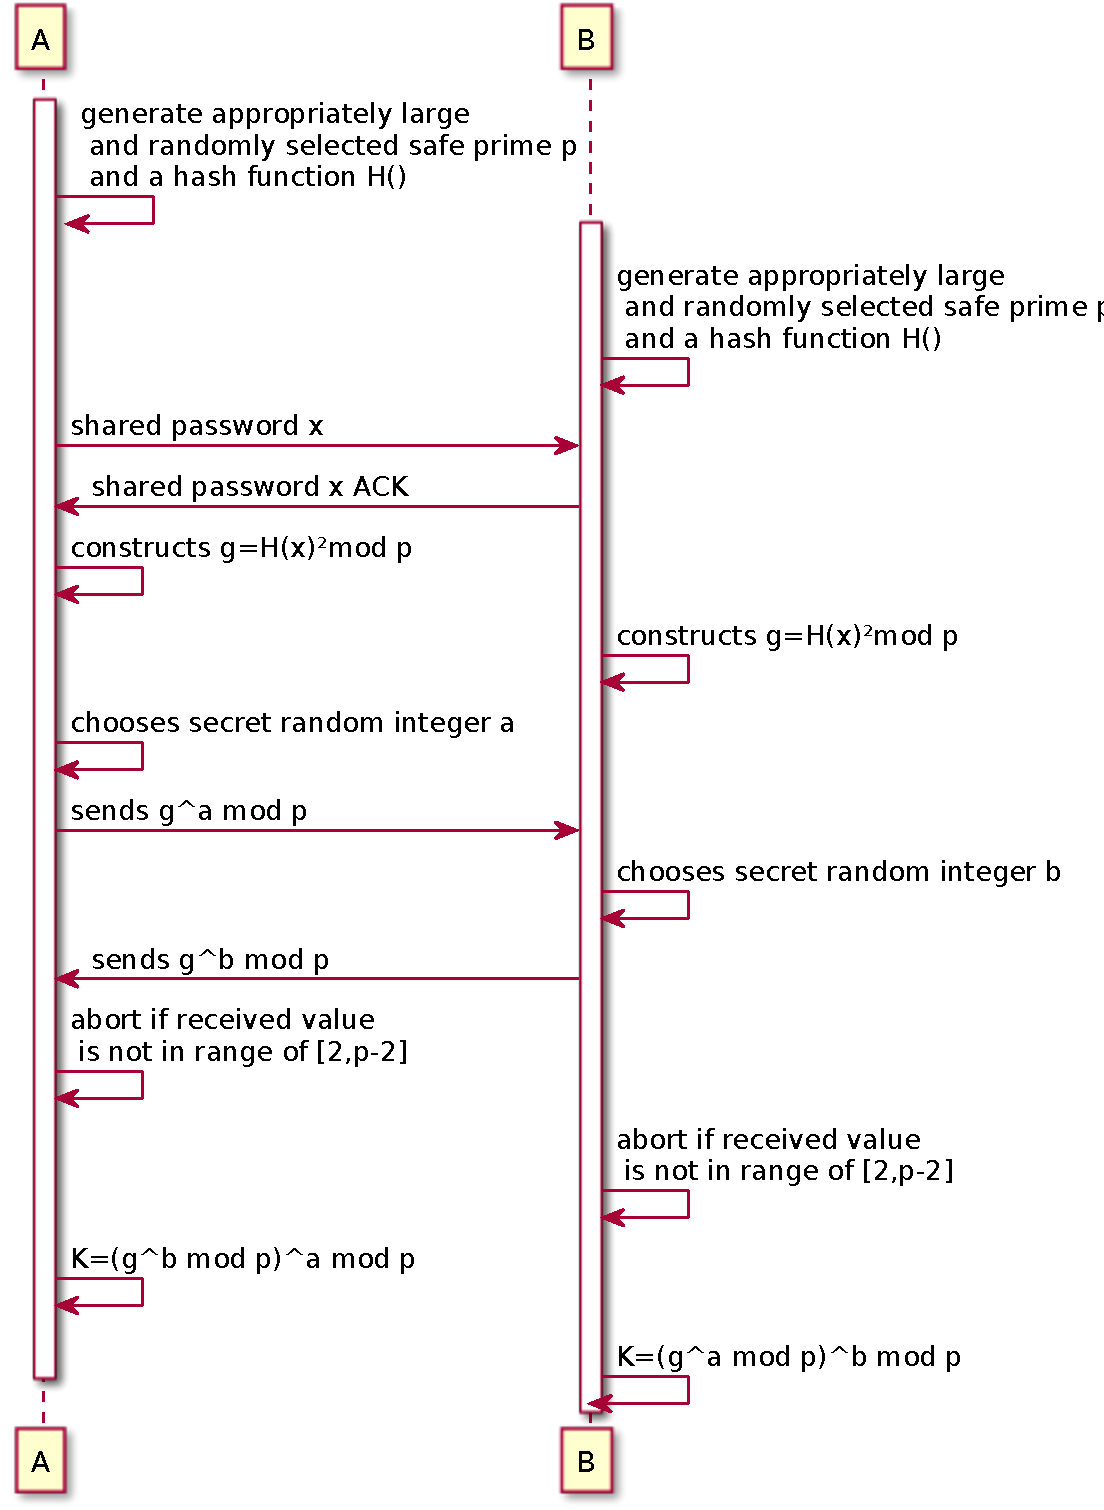
\includegraphics[width = 14cm]{figures/SPEKE.pdf}
			\caption{Sequenzdiagramm Schlüsselaustausch}
		\end{center}
	\end{figure}
	
	\item[Forwarding]
	Die Forwarding-Komponente ist für die interne Weiterleitung von Paketen zuständig.
	Sie koordiniert die Ver- und Entschlüsselung sowie die korrekte Weiterleitung der Pakete an das richtige Ziel.
	Aufgrund dieser Anforderungen muss diese Komponente besonders performant sein.
	Sie ist zudem eine sicherheitskritische Komponente.
	
	\item[Crypto]
	Die Crypto-Kompontene kapselt die Verschlüsselungs-Funktionen, welche das DPDK bereitstellt. 
	Hier wird das AES-GCM verwendet, welches zum Authentifizieren und Verschlüsseln von Paketen genutzt wird. 
	Zudem stellt die Crypto-Komponente die benötigten Funktionen für den Schlüsselaustausch bereit. 
	Sie ist somit eine sicherheitskritische Komponente. 
	Auch muss sie eine hohe Performanz aufweisen.
	
\end{description}

Diese Untergliederung ermöglicht es, das System für Erweiterungen offen zu halten.
In Zukunft wird dadurch auch vereinfacht, eine Unterstützung für weitere Protokolle, zum Beispiel IPv6, hinzuzufügen.

\subsection{Anordnung der Module in Schichten}
Diese Komponenten sind wiederum in einem offenen Schichtenmodell angeordnet.
Die einzelnen Schichten setzen sich folgendermaßen zusammen:
%Grafik für einzelne Schichten einfügen!

\begin{description}
	\item[Verarbeitungsschicht]
	Innerhalb des Frameworks bildet die Verarbeitungsschicht die höchste Abstraktionsstufe.
	Sie beinhaltet das Forwarding-Modul und alle Komponenten, die für das korrekte weiterleiten der Pakete benötigt werden. 
	Dazu zählen insbesondere Forwarding-Tabellen und Schlüsseltabellen.
	Komponenten dieser Schicht dürfen auf die beiden darunterliegenden Schichten zugreifen.
	So kann auf die Kryptofunktionen zugegriffen werden.
	
	\item[Koordinationsschicht]
	In dieser Schicht befinden sich der Dispatcher und der Control Packet Hub. 
	Sie soll das System von allen uninteressanten Faktoren abschotten, indem zum Beispiel Pakete unbekannten Typs verworfen werden.
	Zudem werden einzelnen Komponenten der darüberliegenden Schicht genau die Pakete zugeteilt, die sie verarbeiten können.
	Ebenso werden für nicht performance-kritische Bereiche die Serialisierung der Anfragen übernommen, sodass sich einige Module der höheren Schichten nicht mit Problemen der Thread-Sicherheit auseinander setzen müssen.
		
	
	\item[Abstraktionsschicht]
	Die Abstraktionsschicht wird von der Network Abstraction und dem Crypto-Modul gebildet.
	Ziel dieser Schicht ist es, das in C geschriebene DPDK objektorientiert zu kapseln. 
	Dabei darf jedoch kaum Overhead anfallen.
\end{description}

\clearpage


\section{Verarbeitung verschiedener Pakete}


Um Pakete korrekt weiterleiten zu können, muss PECTO mit verschieden Pakettypen umgehen können. 
Bei der Paketverarbeitung gibt es einen Teil, auf dem alle Pakete gleich behandelt werden, und Abschnitte, die für verschiedene Pakettypen unterschiedlich sind.
Zudem muss unterschieden werden, ob ein Paket aus dem schwarzen oder roten Netz empfangen wurde.

\subsection{Zusammenarbeit zweier Instanzen}
Das einfachste Netz, in dem PECTO zum Einsatz kommen kann, besteht aus zwei roten und einem schwarzen Netz.
Dabei bilden zwei Instanzen PECTOs den Übergang von den roten Netzen ins schwarze.

Schon innerhalb eines solch kleinen Netzes können alle Arten von Paketen auftreten.
Allerdings spielt der gesonderte Umgang mit Broadcast-Paketen erst bei größeren Netzen eine Rolle.

\subsection{Allgemeiner Ablauf beim Empfangen vom Paketen im roten Netz}

Wird ein Paket im roten Netz empfangen, durchläuft es folgende Stufen (siehe Abbildung 2):
\begin{figure}
	\begin{center}
		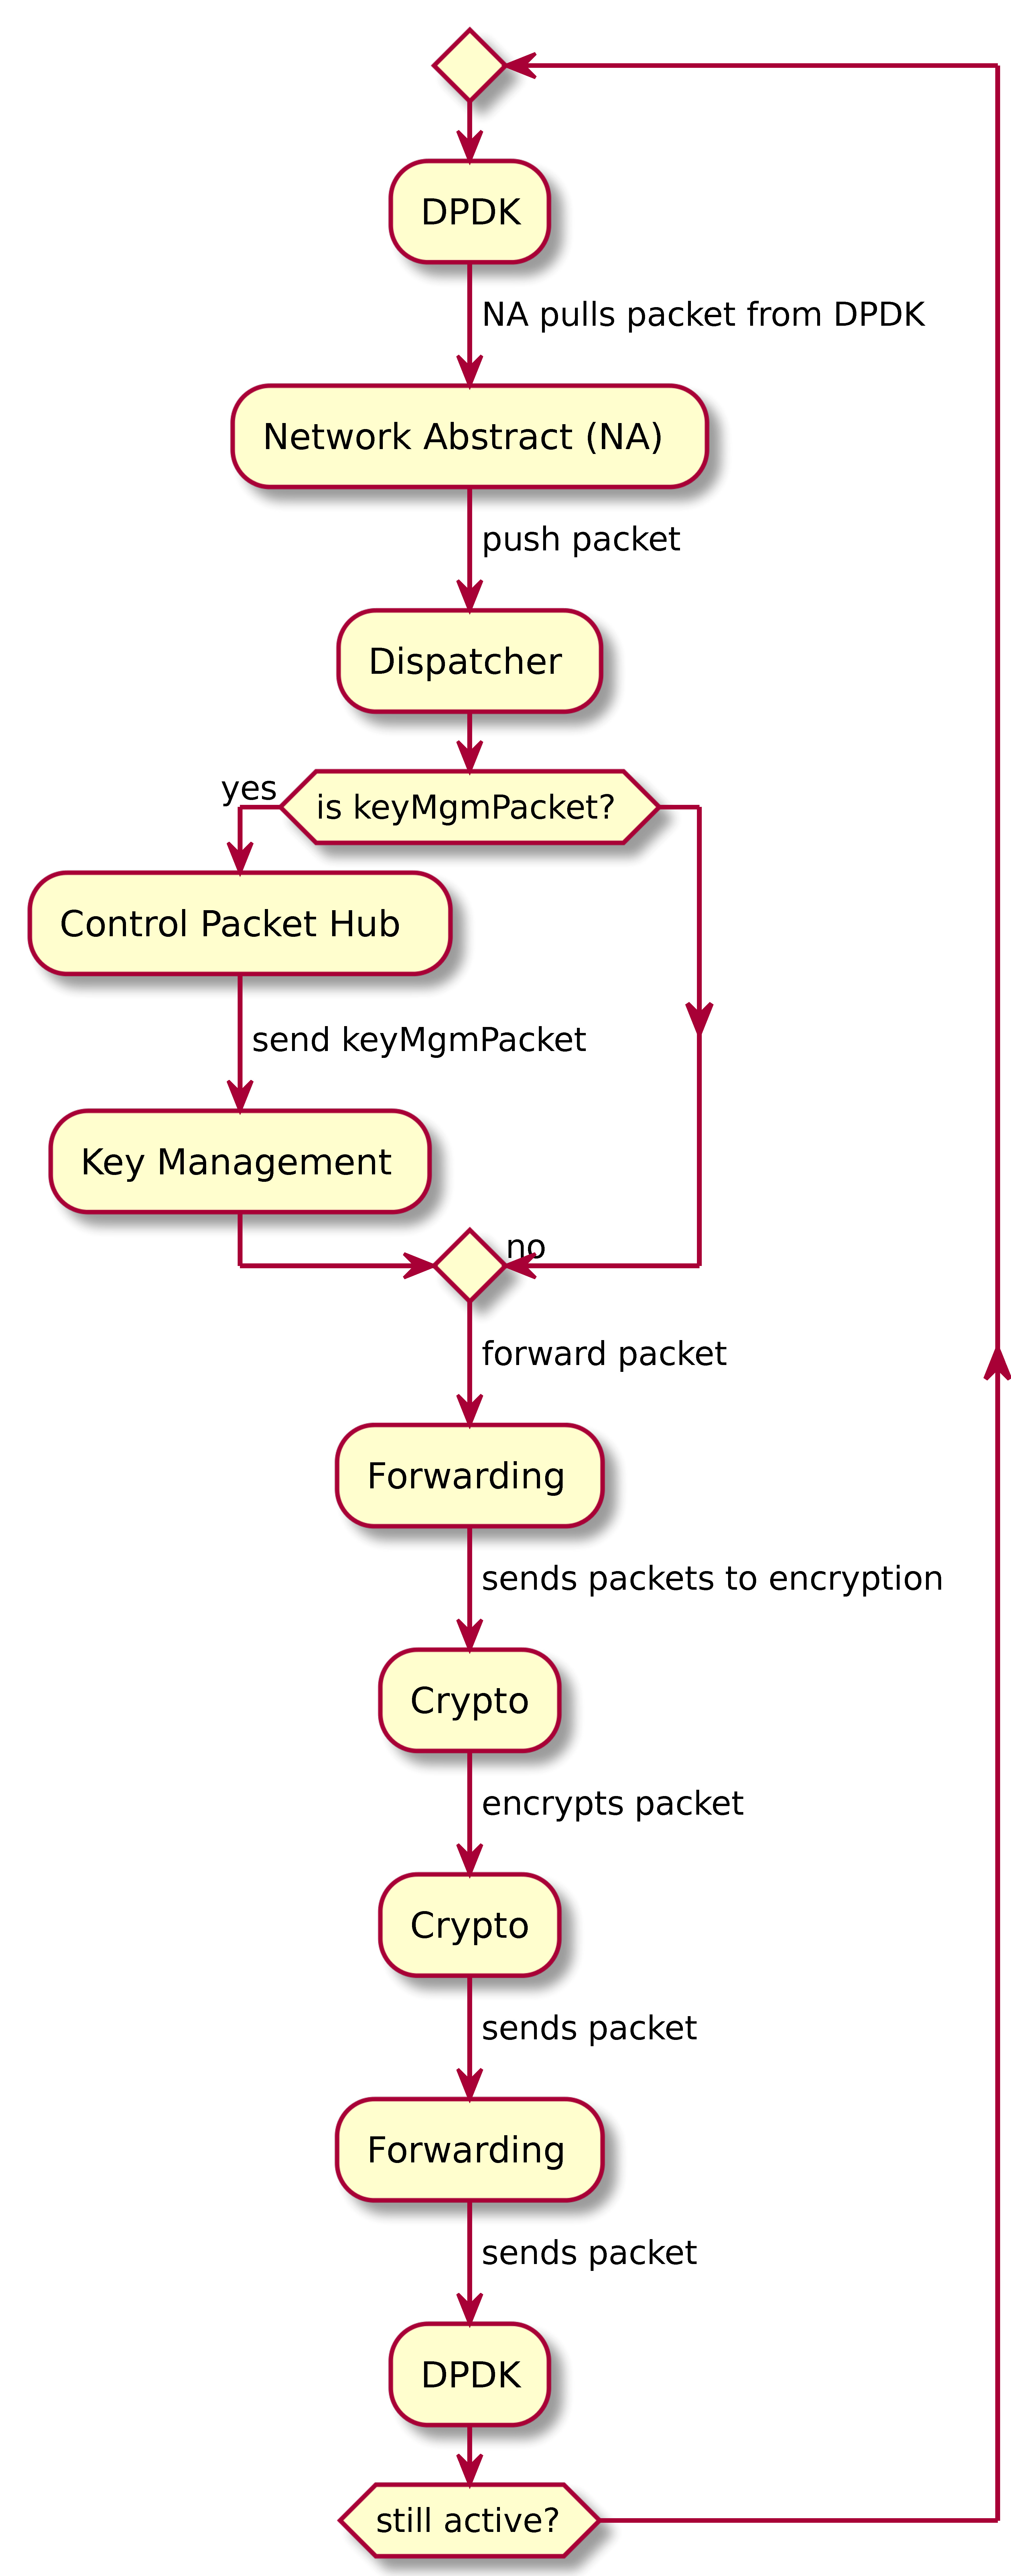
\includegraphics[width = 8cm]{figures/activityDiagram.pdf}
		\caption{Aktivitätsdiagramm}
	\end{center}
\end{figure}



\begin{description}

\item[Empfangen durch das DPDK]
Wenn das Paket von der Netzwerkkarte des Rechners empfangen wird, wird es in eine Empfangswarteschlange geschrieben. 
Von dort wird es mithilfe des DPDKs ausgelesen.
Das Auslesen wird von der Network Abstraction koordiniert.

\item[Dispatching]
Die Netzwerkabstraktionsschicht leitet das Paket direkt zum Dispatch weiter. 
Da es sich um ein Paket aus dem roten Netz handelt, schaut dieses, ob der Pakettyp bekannt ist und verarbeitet werden kann.
Wenn dies der Fall ist, wird das Paket an die Forwarding-Schicht übergeben. (siehe Abbildung 3)

\begin{figure}
	\begin{center}
		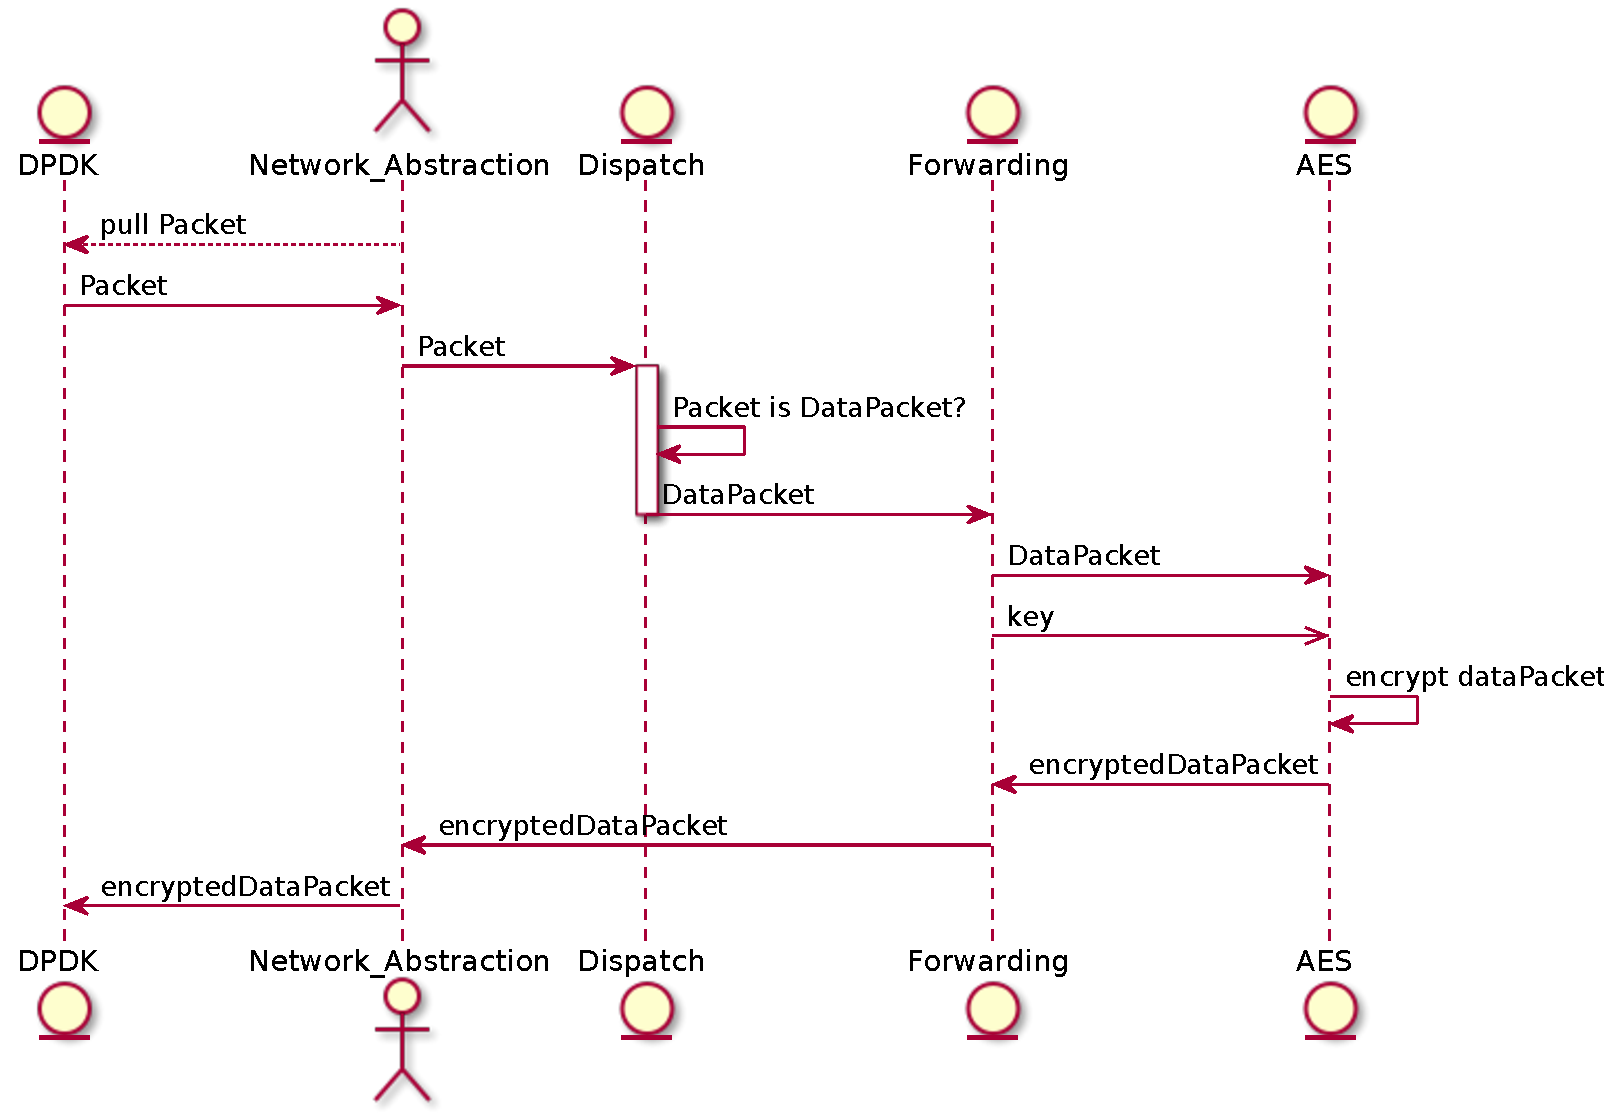
\includegraphics[width = 14cm]{figures/sequenceDiagramDataPacketEncryption.pdf}
		\caption{Sequenzdiagramm Paket Verschlüsselung}
	\end{center}
\end{figure}

\item[Forwarding]
Die Forwarding-Schicht trifft anhand des Pakettyps weitere Entscheidungen über den Umgang mit dem Paket.
Zunächst muss entschieden werden, ob das Paket an eine Gegenstelle weitergeleitet wird.
Dabei wird auch betrachtet, ob das Paket per Unicast an genau eine Gegenstelle übertragen, oder ob Broadcast verwendet wird, um mit allen Gegenstellen zu kommunizieren.
Anhand des Ziels kann entschieden werden, welcher Schlüssel zum Verschlüsseln verwendet wird.

\item[Versenden im schwarzen Netz]
Wenn das Paket verschlüsselt wurde, wird es an das Dispatch weitergeleitet, welches entscheidet, über welchen Netzwerkanschluss das Paket versendet wird.

\end{description}

\subsection{Verarbeitung von IP-Paketen aus dem Roten Netz}

Wird ein IPv4-Paket im roten Netz empfangen, werden in den einzelnen Komponenten folgende Entscheidungen getroffen:

\begin{description}
	\item[Dispatching]
	Das Dispatch erkennt IPv4-Pakete und leitet diese an das Forwarding weiter.

	\item[Forwarding]
	Das Paket wird per Broadcast an alle Instanzen weitergeleitet, wenn es sich um ein IPv4-Broad- oder Multicast-Paket handelt.
	Ansonsten wird in der Forwardingtabelle nachgesehen, ob die Ziel-IP bekannt ist. 
	Wenn dies der Fall ist, wird das Paket an die entsprechende Gegenstelle gesendet.
	Andernfalls wird das Paket verworfen.  
	
\end{description}

\subsection{Verarbeitung von ARP-Paketen aus dem Roten Netz}

Damit das IPv4-Protokoll eingesetzt werden kann, muss auch die Funktionalität vom ARP gewährleistet sein.
Wird ein solches Paket empfangen, treffen die beteiligen Module folgende Entscheidungen:

\begin{description}
	\item[Dispatching]
	Das Dispatch erkennt ARP-Pakete und leitet diese an das Forwarding weiter.

	\item[Forwarding]
	Das Paket wird per Broadcast an alle Instanzen weitergeleitet.
\end{description}

\subsection{Empfangen von Steuerpaketen im schwarzen Netz}

Wird ein Steuerpaket im schwarzen Netz empfangen, durchläuft es folgende Stufen:

\begin{description}
\item[Empfangen durch das DPDK]
Wenn das Paket von der Netzwerkkarte des Rechners empfangen wird, wird es in eine Empfangswarteschlange geschrieben. 
Von dort wird es mithilfe des DPDKs ausgelesen.
Das Auslesen wird von der Network Abstraction koordiniert.

\item[Dispatching]
Die Netzwerkabstraktionsschicht leitet das Paket direkt zum Dispatch weiter. 
Dieses überprüft, ob das Ethernet-Protokollfeld das Paket als PECTO-Steuerpaket ausweist.
Danach wird das Paket zusammengesetzt, falls es sich in mehreren Fragmenten im Speicher befindet. 
Dies ist der Fall wenn das Paket in mehreren Paketen empfangen wird.
Anschließend wird es an den Control Packet Hub weitergereicht.

\item[Control Packet Hub]
Der Control Packet Hub wertet das Paket aus und antwortet gegebenenfalls darauf.
Die Antwort wird an das Dispatch übergeben, der das Paket versendet. 
\end{description}

\subsection{Empfangen von Datenpaketen im schwarzen Netz}

Neben Steuerpaketen werden im schwarzen Netz insbesondere Pakete empfangen, die Nutzdaten enthalten. 
Diese werden entschlüsselt und in das rote Netz weitergeleitet.
Dabei werden folgende Stufen durchlaufen:

\begin{description}

\item[Empfangen durch das DPDK]
Wenn das Paket von der Netzwerkkarte des Rechners empfangen wird, wird es in eine Empfangswarteschlange geschrieben. 
Von dort wird es mithilfe des DPDKs ausgelesen.
Das Auslesen wird von der Network Abstraction koordiniert.

\item[Dispatching]
Die Netzwerkabstraktionsschicht leitet das Paket direkt zum Dispatch weiter. 
Das Dispatch identifiziert das Paket als ein Datenpaket und übergibt es unverändert der Forwardingschicht.

\item[Forwarding]
Die Forwardingschicht versucht, das Paket zu entschlüsseln. (siehe Abbildung 4)
Dabei wird abhängig von den Kopfinformationen des Pakets der Broadcast-Schlüssel oder der Schlüssel des Senders benutzt.
Nach erfolgreicher Entschlüsselung wird überprüft, ob das Paket auch von der angegebenen Quelle versendet werden durfte und ob der gewählte Schlüssel (broad- oder unicast) auch zum Pakettyp passt.
Konnte kein Fehler festgestellt werden, wird das Paket an das Dispatch übergeben, damit es ins rote Netz weitergeleitet werden kann.

\begin{figure}
	\begin{center}
		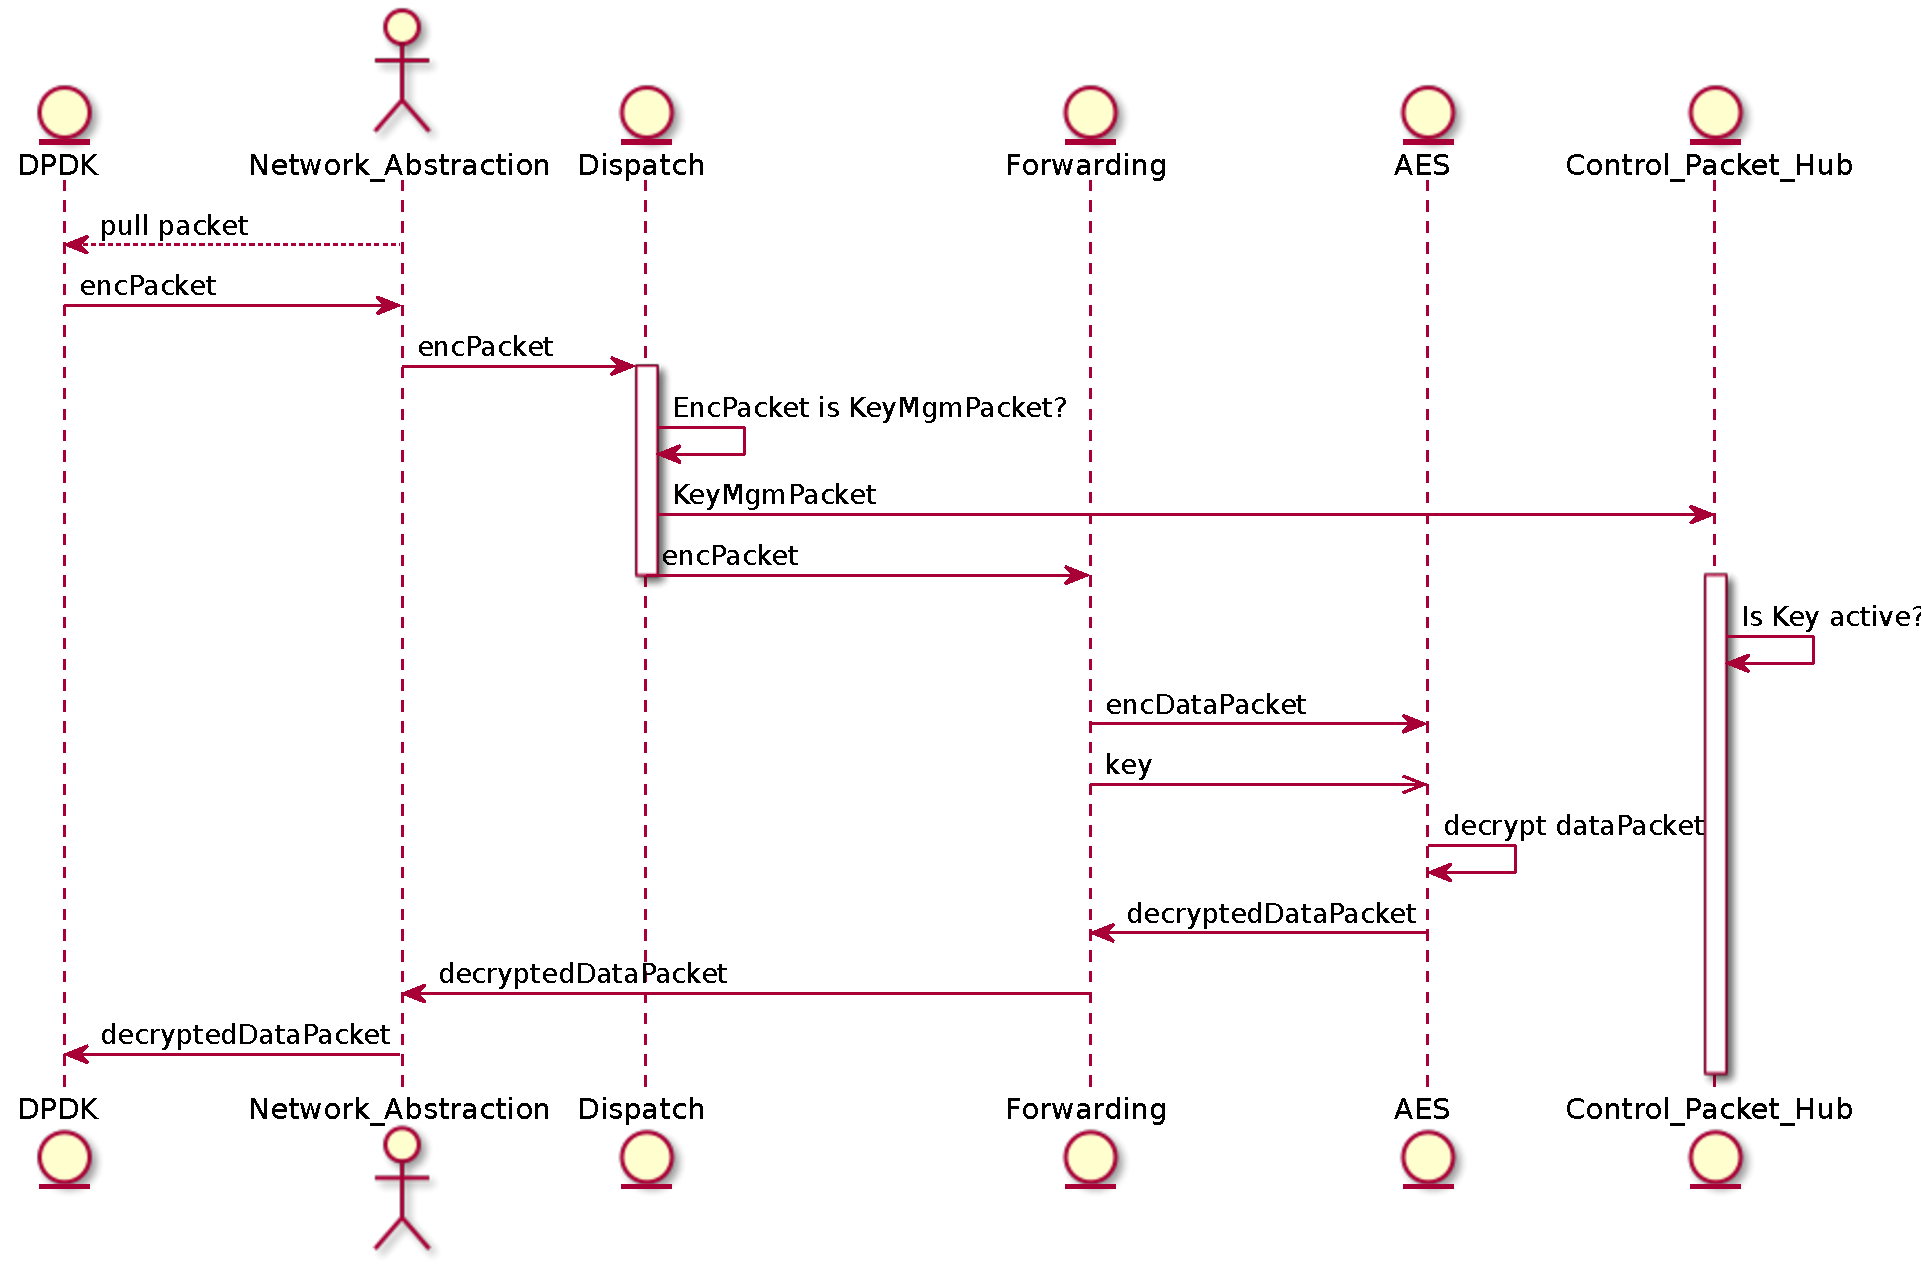
\includegraphics[width = 14cm]{figures/sequenceDiagramDataPacketDecryption.pdf}
		\caption{Sequenzdiagramm Paket Entschlüsselung}
	\end{center}
\end{figure}

\end{description}

\clearpage
\section{Grundlegende Entwurfsentscheidungen}

Durch die Performance- und Sicherheitsanforderungen an das System müssen verschiedene grundlegende Entwurfsentscheidungen getroffen werden.
Dabei konkurriert der Sicherheitsgedanke, der nach möglichst einfachem Code strebt, stets mit dem streben nach hoher Performance.
Um einen guten Ausgleich zu finden, werden alle Komponenten zunächst auf gute Verständlichkeit des Codes optimiert.
Sollten sich beim Profiling Probleme zeigen, werden diese Stellen gezielt überarbeitet.

\subsection{Verwendete Muster}
Zur Realisierung von PECTO werden folgende Entwurfsmuster verwendet:

\begin{description}
	\item[Inversion of Control (IoC)] 
	Um das Schichtenmodell umsetzen zu können und zyklische Abhängigkeiten zu vermeiden, wird Inversion of Control eingesetzt. 
	Die tiefere Schicht stellt dafür jeweils Interfaces bereit, die von den höheren Schichten implementiert werden. 
	Der sich dadurch ergebende Overhead ist in der Regel zu vernachlässigen.
	Insbesondere überwiegen die Vorteile durch eine bessere Entkoppelung.
	Wenn sich Performance-Probleme ergeben, kann davon abgewichen werden.
	
	\item[Exceptions]
	Zur Vereinfachung des Codes werden Exceptions eingesetzt.
	Diese sind immer dann auszugeben, wenn ein unerwartetes Ereignis eingetreten ist.
	Da der Einsatz von Exceptions einen erheblichen Overhead zur Folge haben kann, wenn zu viele von ihnen geworfen werden, müssen für besonders performance-kritische Funktionen immer zwei Schnittstellen zur Verfügung stehen.
	Die erste dieser Schnittstellen löst die Exceptions aus, während die zweite über Rückgabewerte entscheidet ob die Funktion erfolgreich ausgeführt wurde.
	
	\item[Code Contracts]
	Jede Methode, die zu einer öffentlichen Schnittstelle gehört, validiert ihre Parameter und Ausgaben. %wirklich?
	Unerwartete Eingaben, beispielsweise Nullzeiger, müssen erkannt werden und zu einer Exception führen.
	Ebenfalls sollen alle Ausgaben einer einfachen Plausibilitätsprüfung unterzogen werden. 
	Auch hier liegt besonderes Augenmerk auf Nullzeigern.
	So wird sichergestellt, dass keine unerwarteten Rückgabewerte zu Fehlern an anderer Stelle führen können.
	
\end{description}

\subsection{Aufteilung in schnelle und langsame Pfade}

Innerhalb PECTOs ergeben sich zwei verschiedene Pfade, auf denen Pakete verarbeitet werden können.
Einerseits gibt es den besonders performance-kritischen Pfad, den alle Nutzdatenpakete zurücklegen. 
Dieser muss darauf ausgelegt sein, mehrere Millionen Pakete pro Sekunde zu verarbeiten. 
Andererseits müssen Steuerpakete nicht mit der gleichen Effizienz verarbeitet werden, da es von ihnen deutlich weniger gibt.

  
\end{document}
